\section{Integrating multimodal health data for clinical predictions}

\newcommand{\nn}[2]{
    \begin{tikzpicture}
        \node[fill=gray!80, minimum width=3cm, minimum height=2cm, rounded corners=0.1cm, text=white, draw=black, font=\systemfont, anchor=south, text depth=1.5cm] (#2) at (0, 0) {
            #1
        };
        % \draw[-stealth] (input) -- ($ (#2.south west) + (0, 1.25) $);
        % \draw[-stealth] ($ (#2.south east) + (0, 1.25) $) -- (output);
        % \neuron{n00}{($ (#2.south) + (0, 1.25) + (-2*\hsep, -2*\vsep) $)}
        % \neuron{n01}{($ (n00) + (0, \vsep) $)}
        % \neuron{n02}{($ (n00) + (0, 2*\vsep) $)}
        % \neuron{n03}{($ (n00) + (0, 3*\vsep) $)}
        % \neuron{n04}{($ (n00) + (0, 4*\vsep) $)}

        % \neuron{n10}{($ (#2.south) + (0, 1) + (-1.5*\hsep, -1.5*\vsep) $)}
        % \neuron{n11}{($ (n10) + (0, \vsep) $)}
        % \neuron{n12}{($ (n10) + (0, 2*\vsep) $)}
        % \neuron{n13}{($ (n10) + (0, 3*\vsep) $)}

        \neuron{n20}{($ (#2.south) + (0, 0.75) + (-1*\vsep, -1*\vsep) $)}
        \neuron{n21}{($ (n20) + (0, \vsep) $)}
        \neuron{n22}{($ (n20) + (0, 2*\vsep) $)}

        \neuron{n30}{($ (n20) + (\hsep, 0.5*\vsep) $)}
        \neuron{n31}{($ (n20) + (\hsep, 1.5*\vsep) $)}

        \neuron{n40}{($ (n20) + (2*\hsep, \vsep) $)}

        \foreach \j in {0,...,2} {
            \draw[black, opacity=\edgeopacity] ($ (#2.south west) + (0, 0.75) $) -- (n2\j);
        }

        % \foreach \j in {0,...,4} {
        %     \foreach \k in {0,...,3} {
        %         \draw[black, opacity=\edgeopacity] (n0\j) -- (n1\k);
        %     }
        % }
        % \foreach \j in {0,...,3} {
        %     \foreach \k in {0,...,2} {
        %         \draw[black, opacity=\edgeopacity] (n1\j) -- (n2\k);
        %     }
        % }
        \foreach \j in {0,...,2} {
            \foreach \k in {0,...,1} {
                \draw[black, opacity=\edgeopacity] (n2\j) -- (n3\k);
            }
        }
        \draw[black, opacity=\edgeopacity] (n30) -- (n40);
        \draw[black, opacity=\edgeopacity] (n31) -- (n40);
        \draw[black, opacity=\edgeopacity] (n40) -- ($ (#2.south east) + (0, 0.75) $);
    \end{tikzpicture}
}

\begin{frame}{Late fusion: independent insights, combined decisions}
    \begin{tikzpicture}
        \node[draw=black] at (-7, -3.25) {};
        \node[draw=black] at (7, 3.25) {};

        \node[anchor=east, inner sep=0pt] (input2) at (-4, 2.75) {
            {\Huge{\emoji{spiral-notepad}}}
        };
        \node[anchor=east, inner sep=0pt, draw=black] (input) at (-4, 0) {
            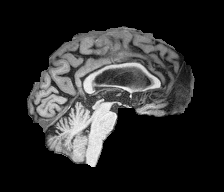
\includegraphics[width=1.5cm]{data/mri_sagittal.png}
        };
        \node[anchor=east, inner sep=0pt] (input3) at (-4, -2.75) {
            {\Huge{\emoji{chart-decreasing}}}
        };
        \only<2>{
            \node[] at (0, 2.25) {
                \nn{EHR-specific ANN}{ehrnn}
            };
            \node[] at (0, 0) {
                \nn{MRI-specific ANN}{mrinn}
            };
            \node[] at (0, -2.25) {
                \nn{MRI-specific ANN}{mrinn}
            };
        }
    \end{tikzpicture}
\end{frame}

\begin{frame}{Early fusion: blending information from the start}
\end{frame}

\begin{frame}{Intermediate fusion: integrating insights along the way}
\end{frame}